% WebAssure project write-up for HackMatrix 2026.
% Compile with pdfLaTeX, for example on Overleaf. Keep the figures folder beside this file.
\documentclass[11pt,a4paper]{article}
\usepackage[T1]{fontenc}
\usepackage[utf8]{inputenc}
\usepackage[scaled=0.95]{helvet}
\renewcommand{\familydefault}{\sfdefault}
\usepackage[a4paper,margin=2.2cm,top=2.3cm,bottom=2.3cm]{geometry}
\usepackage{caption,graphicx,booktabs,tabularx,array,xcolor,enumitem,titlesec,fancyhdr,microtype,float}
\usepackage{xurl}
\usepackage[hidelinks]{hyperref}
\urlstyle{tt}
\definecolor{ink}{HTML}{171717}
\definecolor{muted}{HTML}{6F6F6F}
\color{ink}
\hypersetup{pdftitle={WebAssure: Project Write-up},pdfauthor={Team Fantastic 4}}
\setlength{\parindent}{0pt}
\setlength{\parskip}{6pt}
\setlist{nosep,leftmargin=1.5em,topsep=2pt,itemsep=3pt}
\titleformat{\section}{\Large\bfseries}{}{0pt}{}
\titlespacing*{\section}{0pt}{16pt}{6pt}
\renewcommand{\arraystretch}{1.3}
\pagestyle{fancy}
\fancyhf{}
\renewcommand{\headrulewidth}{0pt}
\fancyfoot[L]{\small\textcolor{muted}{WebAssure | HackMatrix 2026}}
\fancyfoot[R]{\small\textcolor{muted}{\thepage}}
\begin{document}
\begin{center}

\includegraphics[height=.8cm]{figures/logo-hackmatrix.png}\hfill

\includegraphics[height=1.3cm]{figures/logo-acm.png}\hfill

\includegraphics[height=1.15cm]{figures/logo-mlh.png}\hfill

\includegraphics[height=1.4cm]{figures/logo-adamas.png}\hfill

\includegraphics[height=1.1cm]{figures/logo-rice.png}
\end{center}
\vspace{22pt}
{\fontsize{34}{38}\selectfont\bfseries WebAssure\par}
\vspace{4pt}
{\Large Know your website before you trust it.\par}
\vspace{10pt}
{\color{muted} Project write-up for HackMatrix 2026, AI-Powered Web Threat Detection and Digital Trust Intelligence\par
Team Fantastic 4: Souradeep Pradhan, Madhushree Dasgupta, Aniruddha Das and Sattwik Das\par}
\vspace{4pt}

\section{1.\quad Overview}
WebAssure helps people decide whether to trust a link, message or certificate before they act on it. Instead of a bare \textbf{safe} or \textbf{malicious} label, every report shows which checks ran, what each one found, the evidence behind it, what could not be checked and what to do next.

The system combines three layers. \textbf{Cybersecurity} checks collect technical evidence and produce a deterministic risk classification. \textbf{AI} explains that evidence in plain language and analyses scam messages, without being able to change a verdict. \textbf{Web3} records a salted fingerprint of a report on Ethereum Sepolia so anyone holding the receipt can independently verify that it has not been altered.

\section{2.\quad The problem}
Phishing pages, fake job portals, fraudulent payment links and impersonated brands are increasingly hard to tell apart from the real thing. India recorded about Rs 19,813 crore in reported cyber fraud losses in 2025 across roughly 21.78 lakh complaints (I4C data). The Anti-Phishing Working Group counted 971,181 phishing attacks worldwide in the first quarter of 2026.

The trust infrastructure is exposed too. In October 2026, eMudhra disclosed that weak key generation affected eight intermediate certificates, and browser vendors moved to block them. A padlock shows an encrypted connection; it does not prove that a website is honest. People need an explanation they can check, not another opaque score.

\section{3.\quad What we built}
\begin{tabularx}{\linewidth}{@{}>{\raggedright\arraybackslash}p{0.220\linewidth}>{\raggedright\arraybackslash}p{0.540\linewidth}>{\raggedright\arraybackslash}X@{}}
\toprule
\textbf{Capability} & \textbf{What it does} & \textbf{Status} \\
\midrule
URL investigation & Normalises the URL, analyses domain structure and look-alike or homoglyph patterns, follows redirects and inspects DNS, HTTP, security headers and static HTML. & Working \\
TLS and web trust & Verifies the certificate against the system trust store for the hostname and checks leaf key strength and signature hash. & Working \\
Threat intelligence & Checks submitted URLs against Google Safe Browsing, with distinct error states when the provider is unavailable. & Working, needs API key \\
Scam message analysis & Combines a trained classifier with explainable indicators and extracts URLs, phone numbers and email addresses without opening any link. & Working \\
Threat correlation & Connects saved investigations through exact shared domains and leaf certificate fingerprints. Shared indicators never change a verdict. & Working \\
AI explanations & Built-in rule-based explanations cite report evidence. Optional Gemini explanations are schema-validated. & Working \\
Report integrity ledger & Registers salted report fingerprints through MetaMask and verifies receipts independently. & Live on Sepolia \\
Dashboard & Overview, Scans, Messages, Certificates, Threats, Reports, Threat ledger and Settings, with Google and email sign-in. & Working \\
\bottomrule
\end{tabularx}
\vspace{4pt}

\begin{figure}[H]\centering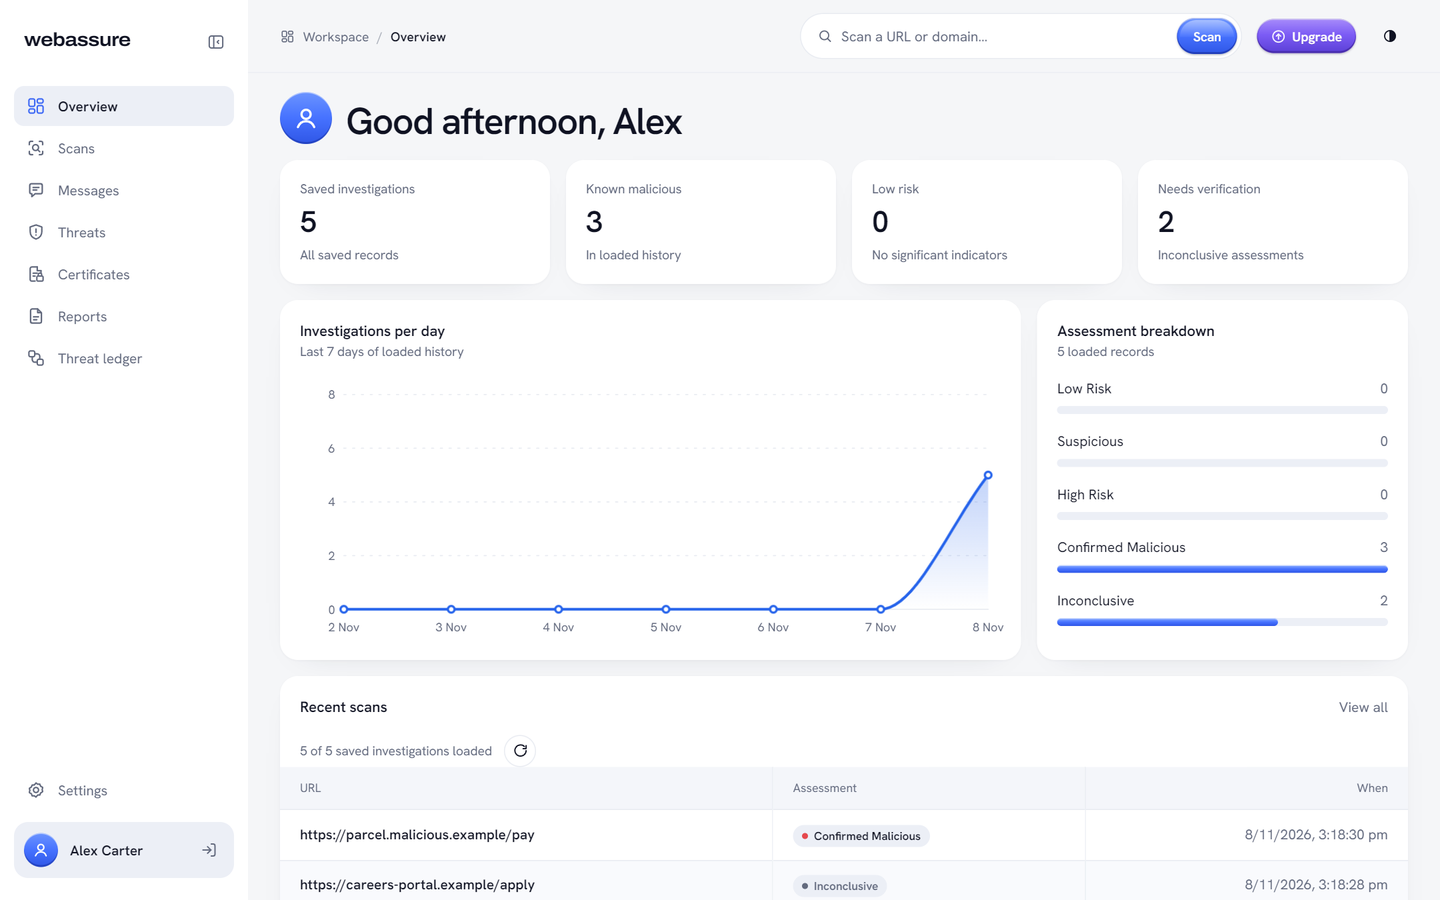
\includegraphics[width=0.86\linewidth]{figures/dashboard.png}
\caption*{\small\textcolor{muted}{WebAssure dashboard, shown with sample scans.}}
\end{figure}
\section{4.\quad Architecture}
\begin{figure}[H]\centering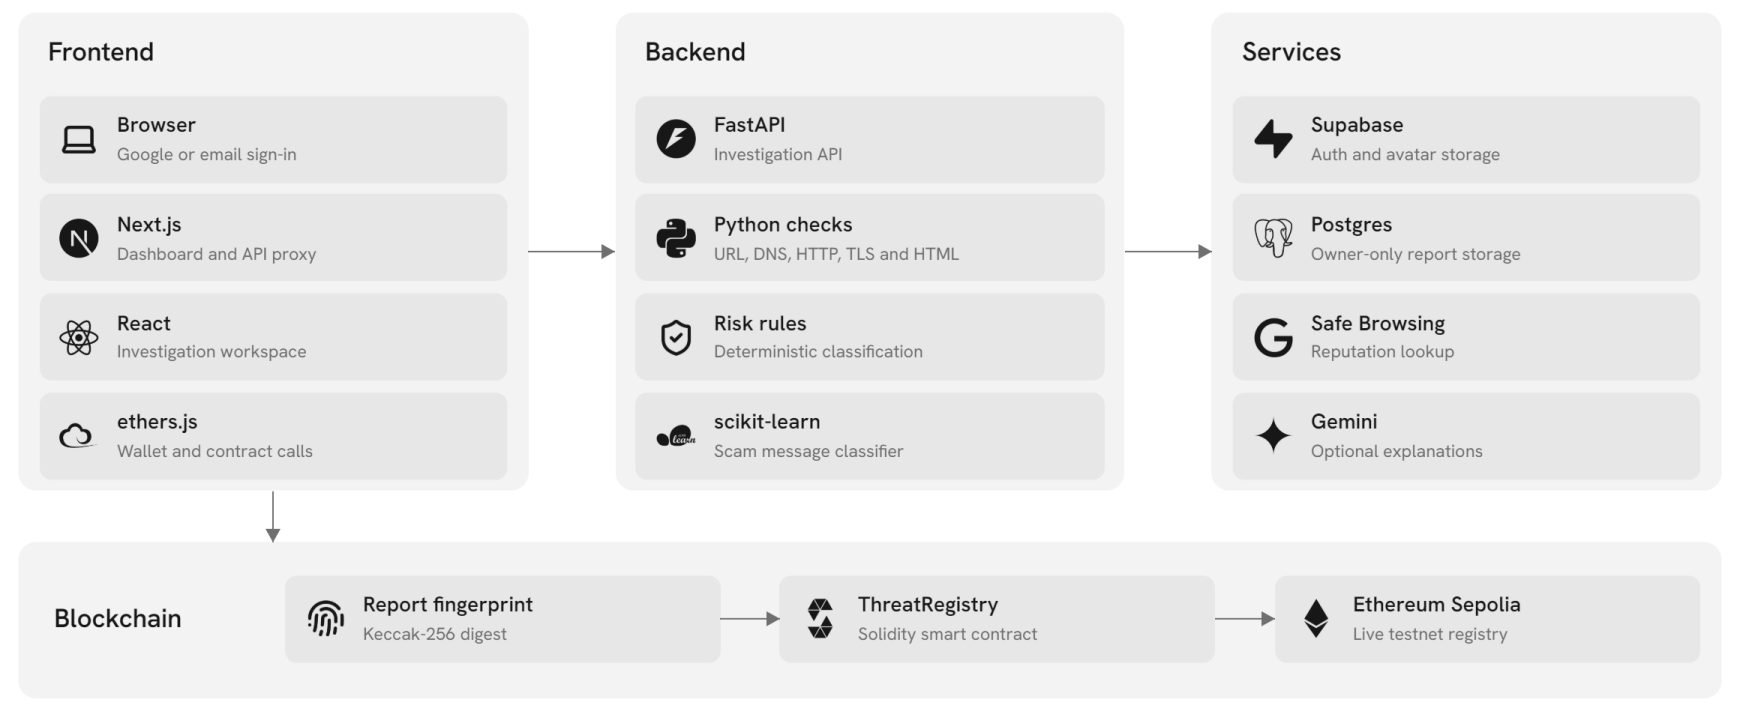
\includegraphics[width=1.0\linewidth]{figures/architecture.png}
\caption*{\small\textcolor{muted}{System architecture.}}
\end{figure}
The browser signs in with Supabase Auth and calls the investigation API through a Next.js proxy. The FastAPI service verifies every bearer token with Supabase Auth, then sends that same user token to PostgREST. Owner filters and Postgres row-level security both restrict access, and the server never holds a service-role key. Wallet and contract calls happen in the browser through ethers.js, so the application never receives a private key.

\section{5.\quad Investigation pipeline}
A submitted URL passes through the following stages. Each stage records its own status, so the final report shows exactly what was and was not covered.

\begin{enumerate}
\item \textbf{Normalise and analyse offline:} URL structure, registrable domain, homoglyph and brand look-alike signals.
\item \textbf{Validate the destination:} resolve DNS and continue only if every address is public.
\item \textbf{Fetch safely, hop by hop:} connect to the validated address, verify TLS and re-validate each redirect, for at most six hops.
\item \textbf{Inspect the response:} security headers and bounded static HTML. Scripts, forms and linked resources are never executed.
\item \textbf{Check reputation:} query Google Safe Browsing for every URL in the chain.
\item \textbf{Classify and explain:} apply the deterministic rules below, then generate an explanation of the evidence.
\end{enumerate}
\textbf{Risk classification.} The first matching rule decides the result. Classifications are not calibrated probabilities, and Low Risk never proves that a website is safe.

\begin{tabularx}{\linewidth}{@{}>{\raggedright\arraybackslash}p{0.210\linewidth}>{\raggedright\arraybackslash}X@{}}
\toprule
\textbf{Classification} & \textbf{Rule} \\
\midrule
Confirmed Malicious & A threat intelligence provider returned a verified match with evidence. \\
High Risk & At least two independent signal groups have significant indicators, and at least one is strong. \\
Suspicious & At least one moderate or strong threat indicator was found. \\
Low Risk & No significant indicators, and all core checks completed. \\
Inconclusive & No significant indicators, but core coverage is incomplete. \\
\bottomrule
\end{tabularx}
\vspace{4pt}

\section{6.\quad AI layer}
\textbf{Message classifier.} Messages are classified with TF-IDF features and Logistic Regression, trained on the 5,574-message UCI SMS Spam Collection with an 80/20 stratified split. Multinomial Naive Bayes was evaluated as a comparison and rejected because of its lower spam recall.

\begin{tabularx}{\linewidth}{@{}>{\raggedright\arraybackslash}p{0.310\linewidth}>{\raggedright\arraybackslash}p{0.135\linewidth}>{\raggedright\arraybackslash}p{0.135\linewidth}>{\raggedright\arraybackslash}p{0.135\linewidth}>{\raggedright\arraybackslash}X@{}}
\toprule
\textbf{Model (1,115-message test split)} & \textbf{Accuracy} & \textbf{Precision} & \textbf{Recall} & \textbf{F1} \\
\midrule
Logistic Regression (selected) & 98.39\% & 94.56\% & 93.29\% & 93.92\% \\
Multinomial Naive Bayes & 96.77\% & 100.00\% & 75.84\% & 86.26\% \\
\bottomrule
\end{tabularx}
\vspace{4pt}

Precision, recall and F1 are for the spam class. These are results on one held-out split of a general SMS spam dataset, not measured real-world scam detection performance, so the classifier is shown alongside explainable indicators.

\textbf{Generated explanations.} Gemini is optional and runs after classification. Evidence is passed to it as untrusted data, URLs in descriptions are stripped, output must match a JSON schema, and it has no ability to change a classification. If Gemini is unavailable, the built-in rule-based explanation is used.

\section{7.\quad Blockchain integrity layer}
A blockchain record can prove that a report has not changed and which wallet registered it. It cannot prove that the report is true, so WebAssure claims only integrity and provenance.

\begin{enumerate}
\item \textbf{Snapshot:} the saved report is frozen together with a random 32-byte nonce, which stops anyone guessing report contents from the public fingerprint.
\item \textbf{Fingerprint:} the snapshot is canonicalised and hashed with Keccak-256.
\item \textbf{Register:} the user approves a MetaMask transaction that sends only the digest to the \nolinkurl{ThreatRegistry} Solidity contract.
\item \textbf{Verify:} verification recomputes the fingerprint and checks the transaction, contract address, registration event, registering address and contract state. It needs no login, application server or wallet signature.
\end{enumerate}
\begin{tabularx}{\linewidth}{@{}>{\raggedright\arraybackslash}p{0.250\linewidth}>{\raggedright\arraybackslash}X@{}}
\toprule
\textbf{Deployment} & \textbf{Value} \\
\midrule
Network & Ethereum Sepolia (chain ID 11155111) \\
Registry contract & \href{https://sepolia.etherscan.io/address/0x5AB0A5fE5026249aDFe1Fb7362C124cdA5296581}{\nolinkurl{0x5AB0A5fE5026249aDFe1Fb7362C124cdA5296581}} \\
Deployment transaction & \href{https://sepolia.etherscan.io/tx/0x94f6a8da67b6f3dc0319b07bb603d0e268f0a61a18773bd84d3a7cf67bb63a10}{\nolinkurl{0x94f6a8da67b6f3dc0319b07bb603d0e268f0a61a18773bd84d3a7cf67bb63a10}} \\
Stored on-chain & Fingerprint, reporter wallet and timestamp only \\
Kept off-chain & The report, its URLs and any personal data \\
\bottomrule
\end{tabularx}
\vspace{4pt}

\section{8.\quad Security and privacy}
\begin{itemize}
\item \textbf{SSRF protection:} only globally routable addresses are allowed, connections go to the validated address, and every redirect is checked again.
\item \textbf{Bounded inspection:} 5-second socket timeouts, a 256 KiB HTML limit, a six-hop redirect limit and four concurrent investigations. Compressed responses and attachments are not read.
\item \textbf{No execution:} no scripts are run, no cookies are sent, and no exploit or intrusive test is attempted.
\item \textbf{Private by default:} reports are owner-only through row-level security. Inaccessible report IDs return 404.
\item \textbf{Prompt injection:} page content and messages are treated as untrusted and cannot influence a classification.
\item \textbf{No sensitive collection:} WebAssure never asks for passwords, OTPs, private keys or seed phrases.
\end{itemize}
\section{9.\quad Challenges we solved}
\begin{tabularx}{\linewidth}{@{}>{\raggedright\arraybackslash}p{0.260\linewidth}>{\raggedright\arraybackslash}X@{}}
\toprule
\textbf{Challenge} & \textbf{How we solved it} \\
\midrule
A failed check must never look clean & Every check reports its own status and coverage. If core checks are incomplete and nothing significant was found, the result is Inconclusive, not Low Risk. \\
Inspecting hostile URLs safely & DNS validation, connecting only to the validated address, re-validation of each redirect, and strict limits on time, size and hops. \\
Keeping AI from overstating evidence & Classification is deterministic and happens first. AI receives evidence as untrusted data, must return schema-valid output, and cannot alter the verdict. \\
Separating suspicion from proof & Confirmed Malicious requires a verified provider match. High Risk requires corroboration from independent signal groups. \\
Publishing proof without leaking data & Only a nonce-salted Keccak-256 digest goes on-chain. Report contents remain in a private receipt held by the user. \\
Multi-user privacy without a privileged key & The API forwards each verified user token, so Postgres row-level security enforces ownership on every request. \\
\bottomrule
\end{tabularx}
\vspace{4pt}

\section{10.\quad Testing}
The repository has \textbf{92 backend tests} and \textbf{23 frontend tests}, all passing at the time of writing. They cover URL analysis, the investigation pipeline, certificates, threat intelligence, explanations, message analysis, the authenticated proxy, correlation and the registry. Registry tests use a real in-memory EVM for deployment, registration, duplicate rejection and tamper detection. Network and provider tests are mocked, so they verify behaviour and do not measure real-world detection accuracy.

\section{11.\quad Limitations}
\begin{itemize}
\item Certificate Transparency and revocation checks are not implemented yet, and each report states this.
\item Automated checks cannot guarantee that a website is safe, and absence of known threats is not proof of safety.
\item The registry is deployed on a testnet. Registration proves integrity and wallet provenance, not the truth of an assessment.
\item Correlation uses exact shared evidence only and does not attribute reports to a campaign.
\item The backend is a local MVP that runs as a single worker.
\end{itemize}
\section{12.\quad What is next}
\begin{itemize}
\item Certificate Transparency, revocation and scheduled certificate monitoring.
\item Validated campaign attribution built on exact shared evidence.
\item A contract audit before moving beyond the Sepolia testnet.
\item Per-user rate limits, data retention controls, network egress restrictions and a durable job queue.
\end{itemize}
\section{13.\quad Disclosures}
\textbf{Open-source software:} Next.js, React, Supabase client, ethers, jsPDF, html-to-image, Solidity compiler, Ganache, FastAPI, Uvicorn, tldextract, confusable-homoglyphs, idna, cryptography, scikit-learn and joblib. \textbf{Services and data:} Supabase, Google Safe Browsing, Google Gemini and the UCI SMS Spam Collection. \textbf{AI tools:} Claude Code assisted with parts of the implementation and documentation, and Google Gemini is part of the product as the optional explanation provider.

\textbf{Source code:} \href{https://github.com/pradhan-not-found/Hackmatrix-26-}{\nolinkurl{github.com/pradhan-not-found/Hackmatrix-26-}}

\end{document}
